\section{Experiment}
\label{sec:exp}

\subsection{Experimental Setup}

\subsubsection{Datasets}
\label{sec:setup_data}
We evaluate our approach on three driving benchmarks. For all datasets, the router is trained exclusively on static detection images and tested on continuous video sequences, without any temporal or tracking supervision at any stage.

\noindent\textbf{KITTI.} 
We train the router on the KITTI Detection dataset~\cite{geiger2012kitti} using an 80:20 split of 5,985 training and 1,496 validation images, and evaluate it on the KITTI Multi-Object Tracking benchmark consisting of 21 video sequences (8,008 frames). 
Frames are processed at a resolution of $384\times1248$.

\noindent\textbf{BDD100K.} 
To evaluate cross-dataset generalization, we train the router on BDD100K detection images~\cite{yu2020bdd} (70K train, 10K val) and evaluate on the BDD100K MOT validation split comprising 200 video sequences. 
Frames are processed at $720\times1280$ resolution.

\noindent\textbf{Waymo Open.}
To further evaluate generalization on a large-scale, high-resolution benchmark, we use the FRONT camera of the Waymo Open Perception dataset~\cite{sun2020waymo} (v2.0.1, modular/parquet release). 
As this benchmark provides no separate detection and tracking splits, we partition it by official split: the router is trained on the 798 training-split segments treated as static detection images (158.1K frames), and evaluated on the 202 validation-split segments as continuous video (39.1K labeled frames).
Frames are processed at $1280\times1920$ resolution.
% Consequently, unlike KITTI and BDD100K---where the image-level router analysis and the final video evaluation use distinct detection and tracking sets---both the image-level calibration (Sec.~\ref{sec:results_calibration}) and the video evaluation here are performed on the same validation split; the training split remains fully disjoint, so no router ever observes its evaluation data.
% Following the official Waymo 2D camera-image detection task, AP is computed (with 2D IoU matching) over the \texttt{vehicle}, \texttt{pedestrian}, and \texttt{cyclist} classes.


\begin{figure*}[!t]
\centering
\begin{minipage}[t]{0.32\textwidth}
\centering
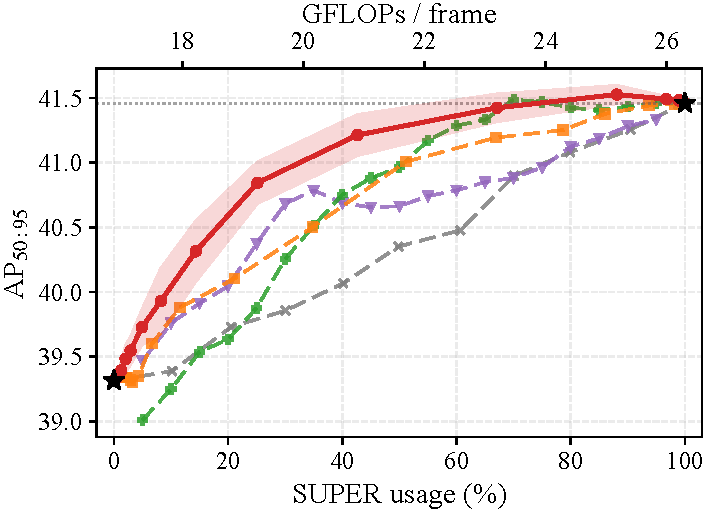
\includegraphics[width=\linewidth]{fig_main_kitti_ap5095.pdf}
\vspace{2pt}
{\small (a) KITTI}
\end{minipage}\hfill
\begin{minipage}[t]{0.32\textwidth}
\centering

\includegraphics[width=\linewidth]{fig_main_bdd_ap5095.pdf}
\vspace{2pt}
{\small (b) BDD100K}
\end{minipage}\hfill
\begin{minipage}[t]{0.32\textwidth}
\centering

\includegraphics[width=\linewidth]{fig_main_waymo_ap5095.pdf}
\vspace{2pt}
{\small (c) Waymo Open}
\end{minipage}
\caption{
    Pareto-front evaluation of depth routing on (a) KITTI-Tracking, (b) BDD100K MOT, and (c) Waymo Open (FRONT camera).
    Each point on the proposed curve corresponds to a different routing threshold $\tau$.
    We compare the advantage-regression router against random, luminance-, edge-density-, and confidence-based routing baselines in terms of AP@[.50:.95] versus SUPER-path usage.
    A single trained router traces a continuous accuracy--efficiency Pareto frontier that consistently dominates all baselines across all three benchmarks, with the largest gains observed in the low-compute regime where SUPER-path execution is limited.
}
\label{fig:main}
\end{figure*}


\begin{table*}[!t]
\caption{
    Efficiency of threshold-based depth routing across the operating points in Figure~\ref{fig:main}. 
    AP denotes AP@[.50:.95] (\%). 
    Latency, FPS, and energy are measured on an RTX~3090 and include router overhead. 
    always-super and always-base represent the static single-path baselines corresponding to the two endpoints of the Pareto frontier.
}
\label{tab:main}
\small
\setlength{\tabcolsep}{2.5pt}
\centering
\begin{minipage}[t]{0.49\textwidth}
\centering
{\small (a) KITTI}\\[2pt]
\footnotesize
\begin{tabular}{lrrrrrr}
\toprule
$\tau$ & SUPER\% & GFLOPs & AP & Latency (ms) & FPS & Energy (mJ)\\
\midrule
\textsc{always-base} & 0.0 & 16.87 & 39.3 & 13.43 & 74.5 & 2099\\
$+0.70$ & 2.9 & 17.14 & 39.5 & 13.91 & 71.9 & 2133\\
$+0.50$ & 8.2 & 17.64 & 39.9 & 14.26 & 70.1 & 2196\\
$+0.40$ & 14.3 & 18.22 & 40.3 & 14.66 & 68.2 & 2268\\
$+0.30$ & 25.1 & 19.24 & 40.8 & 15.38 & 65.0 & 2396\\
$+0.20$ & 42.7 & 20.89 & 41.2 & 16.54 & 60.5 & 2604\\
$+0.10$ & 67.1 & 23.20 & 41.4 & 18.15 & 55.1 & 2893\\
$+0.00$ & 88.1 & 25.18 & 41.5 & 19.54 & 51.2 & 3142\\
$-0.10$ & 96.7 & 25.99 & 41.5 & 20.11 & 49.7 & 3244\\
$-0.20$ & 98.9 & 26.20 & 41.5 & 20.25 & 49.4 & 3270\\
$-0.40$ & 99.6 & 26.27 & 41.5 & 20.30 & 49.3 & 3278\\
\textsc{always-super} & 100.0 & 26.30 & 41.5 & 20.03 & 49.9 & 3283\\
\bottomrule
\end{tabular}
\end{minipage}\hfill
\begin{minipage}[t]{0.49\textwidth}
\centering
{\small (b) BDD100K}\\[2pt]
\footnotesize
\begin{tabular}{lrrrrrr}
\toprule
$\tau$ & SUPER\% & GFLOPs & AP & Latency (ms) & FPS & Energy (mJ)\\
\midrule
\textsc{always-base} & 0.0 & 33.18 & 21.3 & 25.41 & 39.4 & 8312\\
$+0.086$ & 14.8 & 35.92 & 21.8 & 27.86 & 35.9 & 9043\\
$+0.072$ & 26.1 & 38.02 & 22.0 & 29.52 & 33.9 & 9601\\
$+0.064$ & 36.3 & 39.91 & 22.1 & 31.01 & 32.2 & 10105\\
$+0.058$ & 45.8 & 41.66 & 22.2 & 32.41 & 30.9 & 10574\\
$+0.054$ & 55.3 & 43.43 & 22.3 & 33.80 & 29.6 & 11043\\
$+0.049$ & 64.5 & 45.14 & 22.3 & 35.15 & 28.5 & 11497\\
$+0.045$ & 73.0 & 46.72 & 22.4 & 36.39 & 27.5 & 11917\\
$+0.040$ & 81.1 & 48.21 & 22.4 & 37.58 & 26.6 & 12317\\
$+0.033$ & 89.4 & 49.76 & 22.5 & 38.79 & 25.8 & 12727\\
\textsc{always-super} & 100.0 & 51.72 & 22.5 & 40.06 & 25.0 & 13250\\
\bottomrule
\end{tabular}
\end{minipage}

\vspace{8pt}

\begin{minipage}[t]{0.49\textwidth}
\centering
{\small (c) Waymo Open}\\[2pt]
\footnotesize
\begin{tabular}{lrrrrrr}
\toprule
$\tau$ & SUPER\% & GFLOPs & AP & Latency (ms) & FPS & Energy (mJ)\\
\midrule
\textsc{always-base} & 0.0 & 86.46 & 38.3 & 47.77 & 20.9 & 14606\\
$+0.152$ & 13.2 & 92.84 & 38.5 & 52.77 & 18.9 & 16248\\
$+0.116$ & 24.4 & 98.25 & 38.6 & 56.78 & 17.6 & 17640\\
$+0.098$ & 34.6 & 103.21 & 38.7 & 60.43 & 16.5 & 18909\\
$+0.085$ & 44.5 & 108.00 & 38.7 & 63.97 & 15.6 & 20140\\
$+0.074$ & 54.7 & 112.92 & 38.8 & 67.62 & 14.8 & 21408\\
$+0.066$ & 64.0 & 117.43 & 38.8 & 70.95 & 14.1 & 22564\\
$+0.057$ & 73.4 & 121.96 & 38.9 & 74.31 & 13.5 & 23733\\
$+0.048$ & 82.3 & 126.27 & 38.9 & 77.49 & 12.9 & 24840\\
$+0.039$ & 90.4 & 130.19 & 38.9 & 80.39 & 12.4 & 25847\\
\textsc{always-super} & 100.0 & 134.84 & 38.9 & 83.54 & 12.0 & 27041\\
\bottomrule
\end{tabular}
\end{minipage}
\end{table*}


\subsubsection{Baselines}
\label{sec:setup_baselines}

To the best of our knowledge, no prior work has explored depth routing for AnyDepth-style detectors in the image-to-video setting considered here. 
In the absence of established routing strategies, a natural starting point is to rely on human-interpretable notions of scene difficulty. 
One might reasonably expect deeper execution to be more beneficial for visually challenging inputs, such as poorly illuminated scenes, cluttered environments, or frames where the detector exhibits low confidence. 
To benchmark our proposed advantage-regression router against these intuitive cues, we establish the following heuristic baselines:
\begin{itemize}
    \item \textbf{Random Routing:} Selects the execution path randomly based on a target probability, serving as a lower-bound baseline.
    \item \textbf{Luminance-based Routing:} Uses the mean pixel intensity of the input image as the routing signal, operating under the assumption that poorly lit scenes might require deeper execution.
    \item \textbf{Edge-density-based Routing:} Computes the proportion of edge pixels (e.g., via a Sobel operator) in the raw image, acting as a simple pixel-level proxy for scene clutter and object density.
    \item \textbf{Confidence-based Routing:} Uses the detector's own prediction confidence from the previous frame (specifically, the mean score of the top-20 bounding boxes) to decide the path for the current frame, assuming that low confidence indicates a difficult scene.
\end{itemize}



\subsubsection{Implementation Details}
\label{sec:setup_impl}
The router is trained for 30 epochs (batch 256, Adam, lr $10^{-3}$) over seeds 0--4
and reported as mean$\pm$std. 
We do not use weight decay or dropout. 
Furthermore, to maximize training efficiency, the router is trained entirely on precomputed, frozen detector features rather than raw images; therefore, image-space data augmentation is not applied.
Detection uses confidence threshold $0.25$ and NMS IoU $0.7$.


\subsubsection{Evaluation Metrics}
\label{sec:setup_metrics}
We report AP@[.50:.95], the average SUPER-path usage rate, and average GFLOPs per frame over the evaluated video sequences.
We additionally report latency, FPS, and energy consumption measured on an NVIDIA RTX 3090 GPU, including the router forward pass.
% On-device measurements (latency, FPS, energy) include the router forward and are reported against the super-only reference. 



 
%% =====================================================================
\subsection{Results}
\label{sec:results}


 
\begin{figure*}[t]
\centering
\begin{minipage}[t]{0.42\textwidth}
\centering
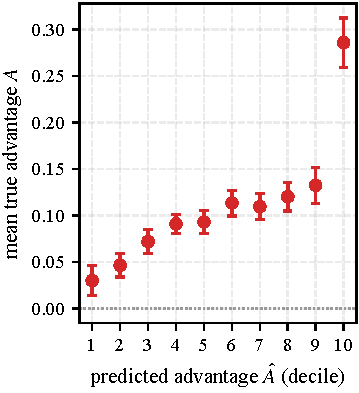
\includegraphics[width=\linewidth]{fig_calibration_kitti.pdf}
\vspace{2pt}
{\small (a) KITTI}
\end{minipage}\hfill
\begin{minipage}[t]{0.42\textwidth}
\centering
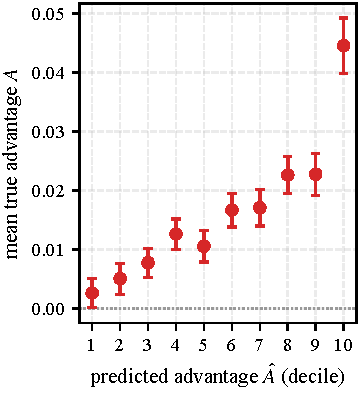
\includegraphics[width=\linewidth]{fig_calibration_bdd.pdf}
\vspace{2pt}
{\small (b) BDD100K}
\end{minipage}
\caption{
    Router ranking reliability. Validation images are grouped into deciles based on the predicted advantage $\hat{A}$ ($5$-seed ensemble). 
    Each point represents the mean true advantage $A=L_{\mathrm{base}}-L_{\mathrm{super}}$ within that decile (error bars denote standard error of the mean). 
    The mean true advantage increases consistently with the predicted decile across both datasets, demonstrating that a higher router score reliably identifies frames that benefit more from the deep path.
}
\label{fig:calibration}
\end{figure*}

\begin{figure}[!t]
\centering

\includegraphics[width=0.9\columnwidth]{fig_advantage_dist.pdf}
\caption{Per-image advantage $A=L_{\mathrm{base}}-L_{\mathrm{super}}$ distribution on
the validation sets. Both are concentrated near zero with a long positive tail---most
frames gain little from the deep path while a minority gain a lot. The tail is wider
on KITTI ($\sigma{=}0.21$) than on BDD100K ($\sigma{=}0.10$).}
\label{fig:adv_dist}
\end{figure}

\subsubsection{Main Result: Pareto Dominance}
\label{sec:results_main}


We compare the proposed advantage-regression router against the heuristic routing baselines. 
Figure~\ref{fig:main} shows that a single trained router traces a continuous Pareto frontier that consistently dominates all baselines across all three benchmarks.
In particular, the advantage of the proposed routing strategy is most pronounced in the low-budget regime, where selecting the right subset of frames for deeper execution is critical.

Table~\ref{tab:main} provides the corresponding operating points along the Pareto curve. 
On KITTI (Figure~\ref{fig:main}(a)), the router maintains AP@[.50:.95] within 0.1 point of the SUPER-only ceiling (41.4 vs.\ 41.5) while routing only 67\% of frames through the SUPER path. 
This reduces computation from 26.30 to 23.20 GFLOPs/frame ($-11.8\%$), latency from 20.69 to 18.66 ms ($-9.8\%$), and energy consumption from 3277 to 2957 mJ ($-9.8\%$), while increasing throughput from 48.3 to 53.6 FPS ($+11.0\%$). 
A more aggressive operating point routes only 43\% of frames to the SUPER path, incurring merely a 0.3 AP reduction while lowering computation by 20.6\%, latency by 18.6\%, and energy by 18.5\%.

The same trend holds on BDD100K (Figure~\ref{fig:main}(b)). 
At 26\% SUPER usage, the router already recovers most of the SUPER-path accuracy gain (22.0 vs.\ 22.5 AP@[.50:.95]) while reducing computation from 51.72 to 38.02 GFLOPs/frame ($-26.5\%$), latency from 39.16 to 28.79 ms ($-26.5\%$), and energy consumption from 13289 to 9669 mJ ($-27.2\%$). 
Throughput correspondingly increases from 25.5 to 34.7 FPS ($+36.1\%$).

The same behavior carries over to the large-scale, high-resolution Waymo Open benchmark (Figure~\ref{fig:main}(c)).
At only 35\% SUPER usage, the router recovers nearly all of the SUPER-path accuracy gain (38.7 vs.\ 38.9 AP@[.50:.95], within 0.2 point of the ceiling) while reducing computation from 134.84 to 103.21 GFLOPs/frame ($-23.5\%$), latency from 16.51 to 14.05 ms ($-14.9\%$), and energy consumption from 2108 to 1677 mJ ($-20.4\%$).
Throughput correspondingly increases from 60.6 to 71.2 FPS ($+17.5\%$).
Notably, the advantage-regression router remains the only strategy that improves monotonically from the very first frames routed to the deep path, whereas the heuristic baselines (most visibly edge density) initially \emph{degrade} accuracy below the always-base anchor by spending the SUPER budget on uninformative frames.



\subsubsection{Advantage Regression Quality}
\label{sec:results_calibration}

Because deployment routes by thresholding the predicted advantage $\hat{A}$, the router need not predict the exact advantage magnitude; instead, it must correctly rank frames according to how much they benefit from the deep path. 
Figure~\ref{fig:calibration} evaluates this property by grouping validation images into deciles based on $\hat{A}$ and reporting the mean true advantage $A = L_{\text{base}} - L_{\text{super}}$ within each group. 
On both datasets, the mean true advantage increases consistently with the predicted decile, indicating that frames assigned higher scores indeed benefit more from deeper execution. 
This confirms that the router successfully captures the relative utility of the deep path, which is the key requirement for threshold-based routing. 
We emphasize ranking rather than per-image regression accuracy because the single-image target is inherently noisy, making robust ordering a more meaningful indicator of deployment performance.

The pronounced increase in the highest decile is explained by the distribution of the true advantage itself (Figure~\ref{fig:adv_dist}). 
The advantage is heavily concentrated near zero while exhibiting a long positive tail, indicating that most frames gain little from deeper execution whereas a small subset benefits substantially. 
The router successfully concentrates these rare high-payoff frames into the top-ranked decile, enabling limited computational resources to be allocated where deeper execution yields the greatest return. 
This positive tail is noticeably wider on KITTI ($\sigma{=}0.21$) than on BDD100K ($\sigma{=}0.10$). 
Accordingly, the advantage distribution on BDD100K spans a much narrower range, as also reflected by the different y-axis scales in Figure~\ref{fig:calibration}, meaning that most achievable operating points are covered by a relatively narrow range of threshold values $\tau$.



\begin{figure*}[t]
\centering
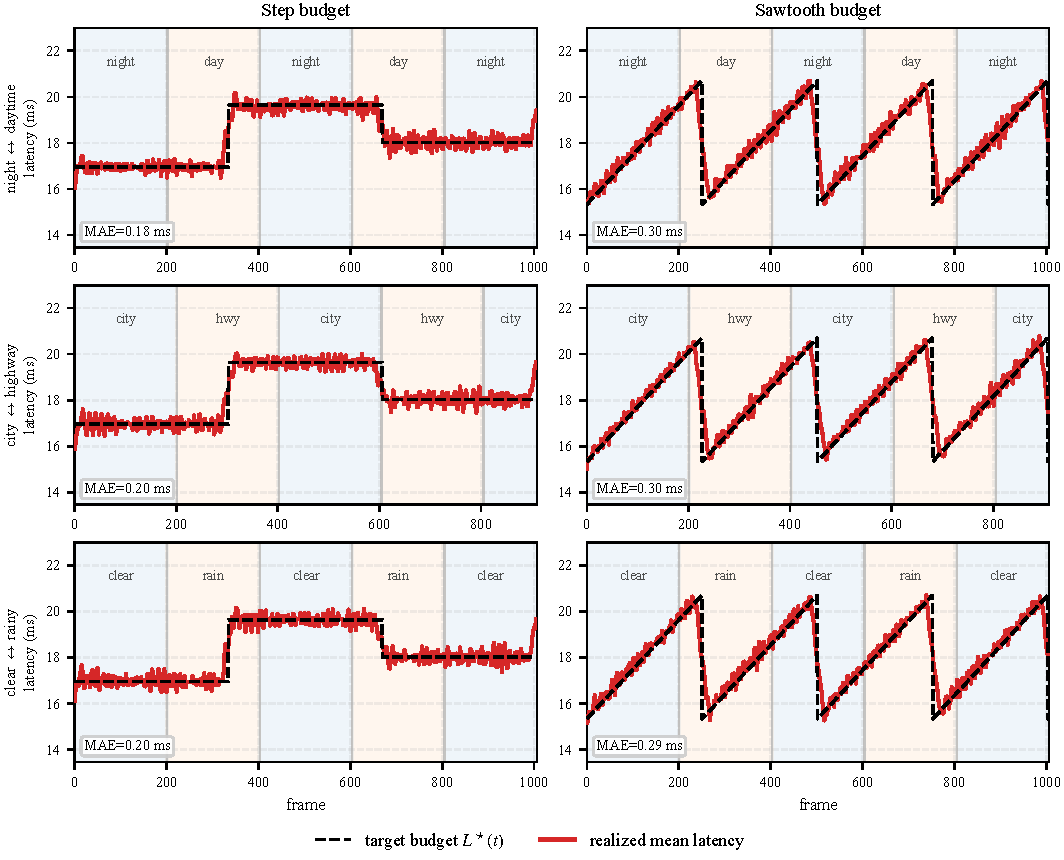
\includegraphics[width=0.85\linewidth]{fig_scenario_budget.pdf}
\caption{
    Runtime latency-budget tracking under realistic scene-condition drift on
    BDD100K MOT, run as a live on-device closed loop.
    Sequences are concatenated in alternating condition order (night$\leftrightarrow$daytime, city$\leftrightarrow$highway, clear$\leftrightarrow$rainy; rows), with shaded bands marking each segment's condition. 
    A PI controller adjusts the router threshold $\tau$ to hold a step (left)
    and a sawtooth (right) latency budget $L^\star(t)$ (black dashed); the realized mean
    latency (red) tracks it with MAE $0.18$--$0.30$\,ms across all condition drifts.
}
\label{fig:budget}
\end{figure*}

\subsubsection{Runtime Latency-Budget Tracking}
\label{sec:results_budget}
The single-scalar threshold $\tau$ exposes the operating point as a tunable dial, allowing the detector to be steered at runtime to track a time-varying latency budget $L^\star(t)$ (e.g., a thermal- or battery-driven schedule) without any retraining. 
We wrap $\tau$ in a proportional-integral (PI) control loop: the controller compares the target budget against an exponential moving average (EMA) of the realized per-frame latency and nudges $\tau$ to cancel the error. 
To stress the controller under realistic non-stationary conditions rather than abrupt synthetic boundaries, we concatenate BDD100K MOT sequences with alternating scene conditions (night$\leftrightarrow$daytime, city$\leftrightarrow$highway, clear$\leftrightarrow$rainy). 
This forces the input distribution---and hence the expected advantage of the deep path---to drift continuously as the scene evolves.

Because individual frames strictly execute at discrete latencies (the super or base), no single frame can exactly match an intermediate target budget. 
Thus, the controllable quantity is the mean latency, effectively the fraction of frames routed to the super path, which the PI controller regulates using the EMA error. 
Figure~\ref{fig:budget} evaluates this runtime tracking as a live on-device closed loop. 
To visualize the tracked mean without the artificial phase delay inherently introduced by causal trailing filters, we smooth the binary per-frame measurements using a zero-phase (centered) moving average. 
This purely offline visualization accurately reflects the controller's tracking quality without smoothing-induced lag, while the underlying closed loop remains unchanged. 
The realized mean latency tracks both step and sawtooth target budgets with exceptional precision across all condition drifts, achieving a mean absolute error of only $0.18$--$0.30$\,ms. 
Ultimately, a single trained router successfully turns a static Pareto front into a robust, runtime-adjustable system that seamlessly adapts to dynamic environments.


%% =====================================================================
\subsection{Ablation Studies}
\label{sec:ablation}
 
\subsubsection{Input Feature: Backbone vs. Neck vs. Both}
\label{sec:abl_feature}

\begin{figure}[t]
\centering
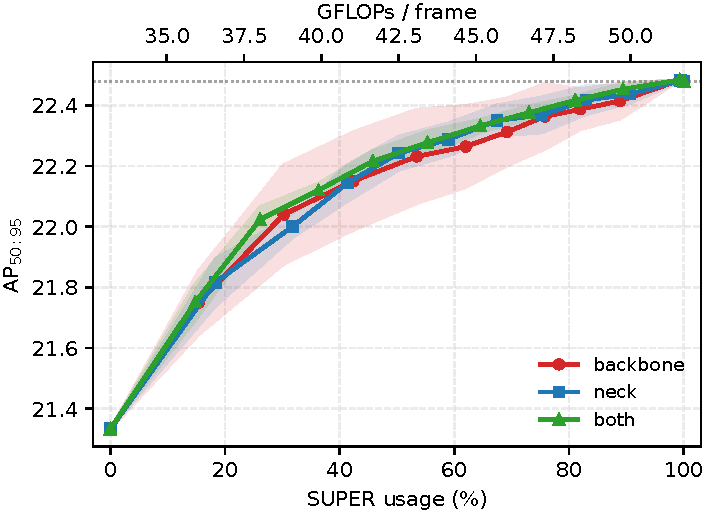
\includegraphics[width=0.9\columnwidth]{fig_abl_feat_ap5095.pdf}
\caption{Feature-source ablation on BDD100K (AP@[.50:.95] vs.\ SUPER usage; mean
$\pm$ std over $5$ seeds). The three sources are close, but the both-feature router
attains the best-or-tied mean with the tightest seed band, whereas backbone-only has
the widest variance.}
\label{fig:abl_feat_source}
\end{figure}

We compare three feature sources for the router on both datasets: the backbone pyramid features (input-level representations, before the detection neck), the neck features (prediction-level representations, immediately before the heads), and their concatenation (both). 

As illustrated in Figure~\ref{fig:abl_feat_source}, the mean accuracy--efficiency trajectories of all three configurations are largely comparable on the BDD100K dataset. 
However, analyzing the performance variance across multiple training seeds reveals a critical distinction in routing stability. 
Relying solely on the backbone yields the widest variance band (red shaded area), suggesting that early-stage representations alone lack the task-specific refinement necessary for consistent advantage prediction. 
Conversely, the concatenation of both feature sets (green curve) consistently attains the best-or-tied mean performance across the entire operational range while exhibiting the tightest variance. 
By providing the router simultaneously with coarse, low-level spatial context from the backbone and refined, task-specific semantics from the neck, the system achieves the most robust routing behavior. 
Given that this concatenation introduces negligible computational overhead (as previously established in Table~\ref{tab:overhead}), we confidently adopt the \emph{both} configuration as our default design.


 
\subsubsection{Router Design and Grid Resolution}
\label{sec:abl_router}

\begin{figure}[t]
\centering
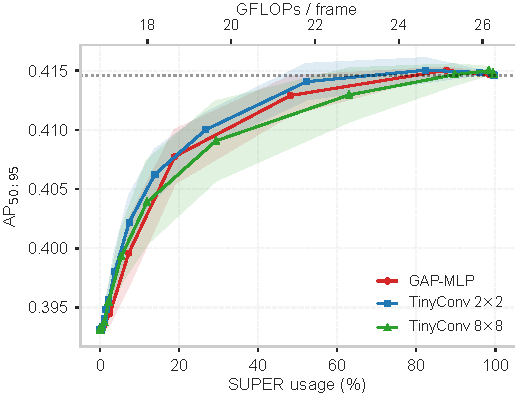
\includegraphics[width=0.9\columnwidth]{fig_abl_router_grid_ap5095.pdf}
\caption{Router design and grid resolution on KITTI. GAP-MLP is compared with
TinyConv at $2\times2$ and $8\times8$ grids in AP@.50:.95.}
\label{fig:abl_router_grid}
\end{figure}

We compare GAP-MLP with TinyConv at $2\times2$ and $8\times8$ grids (Figure~\ref{fig:abl_router_grid}). 
As shown in the performance trajectories, the TinyConv architecture with a coarse $2\times2$ pooling grid consistently achieves the optimal accuracy--efficiency trade-off, outperforming both the spatially-agnostic GAP-MLP and the higher-resolution $8\times8$ variant.
The gap between GAP-MLP and TinyConv $2\times2$ highlights the importance of spatial awareness. 
Because GAP-MLP globally collapses the feature maps, it discards all spatial layout information. 
The superiority of the $2\times2$ grid indicates that preserving a coarse geometric context---allowing the router to roughly distinguish where dense or difficult objects might be located in the frame---provides valuable cues for predicting the advantage of the deep path.
Conversely, increasing the spatial grid resolution to $8\times8$ proves detrimental. 
Not only does it yield the lowest mean performance, but it also suffers from severe instability across varying training seeds, as evidenced by its conspicuously wide variance band (green shaded area). 
This suggests that forcing a lightweight router to process overly fine-grained spatial details causes it to overfit to local feature patterns rather than learning a generalized representation of overall scene difficulty.
Consequently, the $2\times2$ grid emerges as the sweet spot, providing just enough spatial layout to inform routing decisions without introducing the optimization challenges of higher resolutions.


\subsubsection{Previous-Action Sampling Ratio $p(\mathrm{super})$}
\label{sec:abl_prevaction}
During training, we sample the assumed previous action (the path whose features the router conditions on) as \textsc{super} with probability $p$, sweeping $p \in \{0.0, 0.5, 1.0\}$ (Figure~\ref{fig:abl_prevaction}). We find that the balanced setting $p = 0.5$ yields the best performance, outperforming both extreme configurations.
This behavior stems from a train-serve distribution matching effect. 
At deployment, the router must read features produced by whichever path executed on the previous frame, whether it was \textsc{base} or \textsc{super}, and the same image yields slightly different feature maps under each path. 
If training only exposes \textsc{super} path features ($p = 1.0$), the router fails to calibrate to \textsc{base} path features and mis-ranks frames whenever the previous frame ran \textsc{base}. Conversely, $p = 0.0$ fails symmetrically. Training with a balanced $p = 0.5$ exposes the router to both feature distributions equally, ensuring that its advantage prediction remains calibrated regardless of the upstream routing decision. 
The takeaway is that the previous action is an essential component of the router's input distribution, and balanced sampling is vital for robust, causal per-frame deployment.

\begin{figure}[t]
\centering
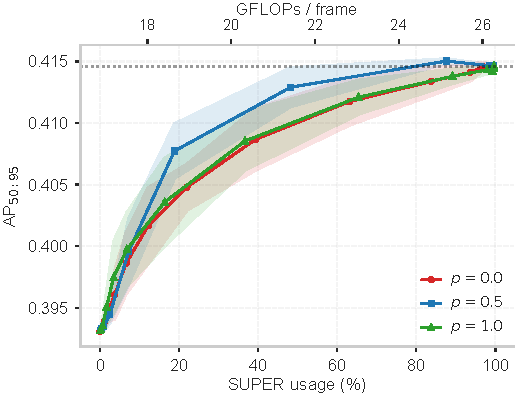
\includegraphics[width=0.9\columnwidth]{fig_abl_prevp_ap5095.pdf}
\caption{Previous-action sampling ratio $p(\mathrm{super})$ during training
(AP@.50:.95) on KITTI.
}
\label{fig:abl_prevaction}
\end{figure}


